%=================
\chapter{Sprint 4}
%=================
This chapter describes the work done in sprint 4. The 
chapter is divided into sprint planning in \autoref{sec:sp4:planning}, design 
made in the sprint in \autoref{sec:sp4:design}, the implementation in 
\autoref{sec:sp4impl}, the result of the sprint testing in 
\autoref{sec:sp4test}, feedback from the customer in 
\autoref{sec:sp4feedback} and evaluation of the sprint in 
\autoref{sec:sp4eval}.

%------------------------
\section{Sprint Planning}
%------------------------
\label{sec:sp4:planning}
The fourth sprint will be the last iteration of this project.
The sprint work hours will be split between implementing new features,
improving existing features and making sure the \gls{utility} work properly
on Thales' source code.

Before the sprint the customer tried our \gls{utility} on close to 200 C
header files, but was only able to generate four \glspl{dissector}.
For the \gls{utility} to be of value to Thales we must improve this.

Feedback from the customer before sprint 4 revealed that certain requirements
were not fulfilled, and needed to be improved. These were added as work items
to this sprint backlog in \autoref{tab:sprint4req}. In addition, we received new
requirements that the customer would like us to implement.

As this is the last sprint, and with the new requirements from the customer it
is clear we will not be able to complete them all. We made some of the new
requirements optional as we only allowed 350 work hours of tasks in the sprint
backlog. We are trying to improve the process by only adding tasks which we
can complete during the sprint. We are prepared to work more for any new tasks
and unforeseen bugs we must fix.

We have agreed to write suggestions on how to implement any optional tasks
not completed during the sprint.

\subsection{Duration}
%-----------------------
The sprint started with the planning meeting the 2nd of November and our work started the following day. The sprint duration is 14 days, and will end on the 15th of November with a review meeting. 

\subsection{Sprint Goal}
%-----------------------
The goal of this sprint will be to focus on fixing and implementing functions that the customer will need to use the \gls{utility} on their source code. The most important thing to focus on in the beginning of the sprint will be to implement support for \#pragma directives and support for including \gls{header}-files that are not included by the \gls{preprocessor}. This is important, as it will make it possible for the customer to fully test the \gls{utility}.

Since the deadline of the project is 24th November, there will also be a focus on preparing a presentation and improving the report for the final delivery. The team are also going to hold a presentation for the customer's developers on the 17th of November, and it is important to also focus on this presentation.

\subsection{Back Log}
%--------------------
This section contains the sprint backlog in \autoref{tab:sprint4req} and the timetable for the sprint in \autoref{tab:sprint4time}.  

\begin{table}[htbp] \small \center
\caption{Sprint 4 Requirement Work Items \label{tab:sprint4req}}
\begin{tabularx}{\textwidth}{l X c c}
	\toprule
	User & & \multicolumn{2}{c}{Hours} \\
	\cmidrule(r){3-4}
	story & Req. and Description & Est. & Act. \\
	\midrule
	\textbf{Impl.} &  & \textbf{47} & \textbf{24} \\
	US56 & FR2-E: Guess \gls{dissector} from \gls{packet} size & 5 & 3 \\
 	US40 & FR3-A mod: Support \gls{include} of system \glspl{header} &  8  & 3 \\
	US41 & FR3 mod: Ignore \#pragma directives & 2 & 1 \\
	US42 & FR3-A mod: Find include dependencies which are not explicitly set & 16  & 11 \\
	US47 & FR4-B mod: Custom \Gls{lua} files support inside a .cnf file & 4 & 1 \\
	US49 & FR4-D mod: Multiple message ID's for one \gls{dissector} & 2 & 1 \\
	US53 & FR4-H:Automatic generation of placeholder configuration & 1  & 0.5\\
	US51 & FR4-I: Support specifying the size of unknown struct members & 4 & 1 \\
	US43 & FR6-E: Support C \#defines and --Include from CLI & 1 & 1 \\
	US54 & FR6-F: Only generate dissectors for structs with valid ID & 4 & 1.5 \\
	\addlinespace
	\textbf{Fixes} &  & \textbf{35} & \textbf{43.5} \\
	& TheFIX: Be able to process customer's files & 12 & 17 \\
	 & FR2-A: Improve generated \Gls{lua} output & 10 & 20 \\
	 & FR1-E: \Gls{array} bug in text & 2 & 1.5 \\
	 & FR1-E: Pointer support (array) & 1 & 0.5 \\
	 & FR1-E: \Gls{enum} in \glspl{array} & 1 & 1 \\		
	 & FR6-C: \Gls{batch mode} (recursive search for subfolders) &  8  & 2 \\
	 & FR6-C: Support command line arguments for Cpp & 1 & 0.5\\
	 & Exclude certain folders and files in batch mode & 1 & 1 \\
	\addlinespace
	\textbf{Testing} &  & \textbf{16} & \textbf{7.5} \\
	 & Fixing existing tests & 3 & 3.5 \\
	 & Add more tests for csjark module & 3 & 1 \\
	 & Add more tests for cparser module & 3 & 0.5 \\
	 & Add more tests for the config module & 2 & 0.5 \\
	 & Add more tests for the dissector module & 2 & 0.5 \\
	 & Add more tests for platform module & 1 & 0 \\
	 & Add sprint 4 end-to-end tasks & 2 & 1.5 \\
	\addlinespace
	\textbf{Doc.} &  & \textbf{15} & \textbf{17.5} \\
	US44 & Update command line interface document & 1 & 1 \\
	US48 & Update user documentation for custom \Gls{lua} & 1 & 1.5 \\
	US50 & Update user documentation for message ID & 1 & 1 \\
	US52 & User documentation for \gls{struct} size configuration & 1 & 1 \\
	US55 & User documentation for generating only \gls{struct} with valid ID or dependencies & 1 & 1 \\
	US36 & Which platforms that the \gls{utility} supports & 2 & 1 \\
	US58 & How to define new platforms to support & 1 & 3.5 \\
	US37 & Create developer manual from python docstrings & 2 & 2 \\
	& Updates and polishing & 5 & 5.5 \\
	\midrule
	& Total: & 113 & 92.5 \\
	\bottomrule
\end{tabularx}
\end{table}

\begin{table}[htbp] \small \center
\caption{Sprint 4 Timetable\label{tab:sprint4time}}
\begin{tabularx}{\textwidth}{X c c}
	\toprule
	& \multicolumn{2}{c}{Hours} \\
	\cmidrule(r){2-3}
	Description & Est. & Act. \\
	\midrule
	\textbf{Sprint planning} & \textbf{30} & \textbf{27} \\
	\addlinespace
	\textbf{Sprint 4 requirements} & \textbf{113} & \textbf{92.5} \\
	Implementation & 47 & 24 \\
	Fixes & 35 & 43.5 \\
	Testing & 16 & 7.5 \\
	User Documentation & 15 & 17.5 \\
	\addlinespace
	\textbf{Sprint review} & \textbf{20} & \textbf{20} \\
	\addlinespace
	\textbf{Sprint documentation} & \textbf{46} & \textbf{52.5} \\
	Sprint 3 document & 4 & 4 \\
	Sprint 4 document & 42 & 48.5 \\
	\addlinespace
	\textbf{Report work} & \textbf{38} & \textbf{49} \\
	Update tables with actual hours & 2 & 2 \\
	Abstract - improve & 2 & 3\\
	Importing user documentation to report & 3 & 11 \\
	Introduction section & 6 & 10 \\
	Report read-through from a technical perspective & 6 & 6\\
	Report read-through from a non-technical perspective & 6 & 7\\
	Glossary refinement & 3 & 3\\
	Acronym refinement & 1 & 1\\
	Write about optional requirements & 4 & 2\\
	References & 3 & 2\\
	Requirement agreement & 2 & 2\\
	\addlinespace
	\textbf{Thales presentation} & \textbf{28} & \textbf{28} \\
	\addlinespace
	\textbf{Meetings} & \textbf{63} & \textbf{48.5} \\
	Advisor meetings & 28 & 20 \\
	Customer meetings & 14 & 10 \\
	Stand-up meetings & 21 & 18.5 \\
	\addlinespace
	\textbf{Project management} & \textbf{17} & \textbf{27} \\
	\midrule
	Total: & 351 & 344.5 \\
	\bottomrule
\end{tabularx}
\end{table}


%----------------------
\section{System Design}
%----------------------
\label{sec:sp4:design}
At the start of the fourth sprint our utility was only able to successfully
parse a few of the header files in the customer's code base. We had to add
functionality to support corner cases of features we already had, and to
remove C code which \gls{pycparser} does not accept, like \#pragma directives.

This sprint the design will not be as comprehensive as in prior sprints, for two reasons:
\begin{itemize}
	\item This was the last sprint, if we were to implement many new features we also had to use time for testing and writing documentation for them, which we did not have.
	\item The existing features had to be extensively tested and documented before the project was over, leaving less time for other work. Testing and bug fixing was essential this sprint.
\end{itemize}
After three sprints, the design was to a large degree set. To make the
individual modules less complex, we re-factored some code and introduced
some new modules, which is described below.

\subsection{System overview}
%---------------------------
The addition of new requirements from the customer resulted in changes in the utility's system overview. The need for more custom handling resulted in a re-factoring of the code. This is visible in the class diagram in \autoref{fig:sp4class}, which was extended from the third sprint. Two new modules was added, cpp and field. Major changes to the class diagram are described below. How the modules interact is described in \autoref{sec:sp4:design:md}.

\begin{figure}[htbp]
	\noindent\makebox[\textwidth]{%
	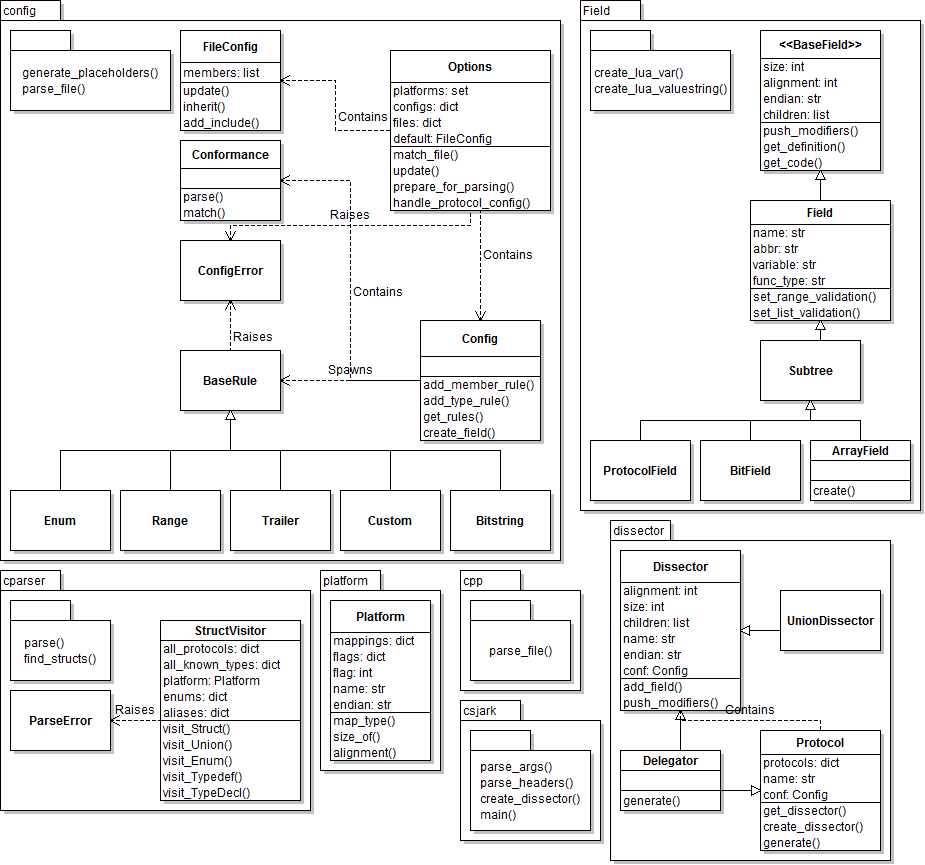
\includegraphics[width=1.2\textwidth]{./sprints/img/ClassDiagramSprint4v2}}
	\caption{Sprint 4 Class Diagram \label{fig:sp4class}}
\end{figure}

\subsubsection{ccp module}
The need for preprocessing C files before they are parsed have become so comprehensive, that we decided to create a dedicated module for it. All the existing cpp concerned code was relocated from the cparser module, and joined with the new implementation. The requirements listed in\autoref{tab:sprint4req}, made it necessary to have more functionality regarding the preprocessor step. Especially we need to remove parts of the output of the C preprocessor before forwarding it to the \gls{pycparser} library.

\subsubsection{field module}
Field specific classes were moved from the dissector module to its own module, field. For the same reason as the ccp module; the amount of code concerning fields became so large, that an own module was appropriate. There was some refactoring in the field module. An interface, BaseField, was added and has Field as a subclass. The class Field is the most important class in this module, and generate code for most of fields used by dissector. Subtree is a class that generates fields for the dissector, that will need a subtree in Wireshark, this class has three subclasses, BitField, ArrayField and ProtocolField.

\subsubsection{cparser module}
Some changes was done in this module due to the refactoring, functionality for C preprocessing was moved, and some new methods was added. 

\subsubsection{config module}
The class FileConfig was added, to hold the configuration for specific header-files. Some methods was also added for automatic generation of header-files.

\subsubsection{dissector module}
There was several changes, all the Field classes was added to it's own module.
The Dissector-class was added, which holds fields representing one struct for
a specific platform. Protocol is now a collection of Dissectors, one for each
platform. UnionProtocol was renamed to UnionDissector.

\subsection{Module Diagram}
%--------------------------
\label{sec:sp4:design:md}
\autoref{fig:sp4module} shows the dependencies between the modules. The main 
module for the utility is csjark, which have the main-method. This module 
uses config to parse and hold all the configuration, starts preprocessing in 
cpp module, and then uses cparser to parse the header files which returns
all the generated protocols. At the end the dissector module generates
Lua dissectors, which the csjark module writes to files.

The cpp module uses the config module to read options given for the c 
preprocessing.

The config module uses the two modules field and dissector to create 
configured dissector fields and the delegator class.
The platform module is read, to get de predefined platform configurations.

When the cparser have parsed a header file it traverses the abstract syntax
tree to create Protocol instances which represents Structs and Unions. To do
this the cparser module depends on four modules: config, platform, dissector
and field.

The dissector module uses the field module to generate fields for all the 
struct members. It also uses the platform module to a list of all platforms
to support.

The field module depends on the platform module to test if field endian is big
or little.

\begin{figure}[htbp]
	\center
	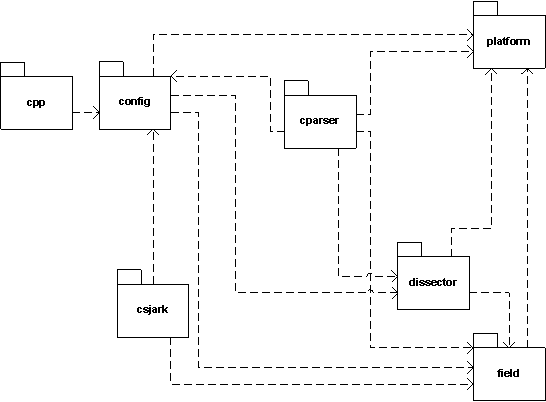
\includegraphics[width=\textwidth]{./sprints/img/sp4modulediagram}
	\caption{Sprint 4 Module Diagram \label{fig:sp4module}}
\end{figure}

\subsection{User Stories}
%------------------------
\label{sec:req:stories4}
This section lists the user stories for the fourth sprint, these are displayed in \autoref{tab:req:stories11}, \autoref{tab:req:stories12}, \autoref{tab:req:stories13} and \autoref{tab:req:stories14}.
These user stories represent how we intend to add the functionality of each requirement of the fourth sprint,
and contains information on how the modules of CSjark should interact with each other.
Some of the user stories explains how the user documentation should be written, while one of them explains the modification of the \gls{include} requirement we implemented in sprint 1.

\begin{table}[htbp] \footnotesize \center
\caption{User Stories - Sprint 4 Part 1\label{tab:req:stories11}}
\noindent\makebox[\textwidth]{%
\begin{tabularx}{1.2\textwidth}{l X}
	\toprule
	Header & Value \\
	\midrule
	ID & US40 \\
	Requirement & FR3-A modification: \gls{include} system includes \\
	What & The \gls{utility} needs to support system dependent \gls{header}-files
	even if these are not available on the platform that the \gls{utility} is used on. \\
	How & The administrator is able to specify a fake system \gls{header} file with the defines they need to make their \glspl{struct} work correctly.
	This fake \gls{header} is then used to represent the system \gls{header} in the file so it is parsed correctly by \gls{pycparser}.  \\
	Result & The administrator is now able to make the \gls{utility} generate system dependent \glspl{dissector} for \glspl{header} with system dependent includes. \\
	\midrule
	ID & US41 \\
	Requirement & FR3 modification: Ignoring \#pragma directives \\
	What &  The \gls{utility} needs to be able to support \gls{header} files with the \#pragma directive without necessarily having to support the functionality of the directive\\
	How & Before feeding the \gls{header} files to the \gls{parser}, the \gls{utility} needs to be able to run a pass through all of the \glspl{header} that are to be parsed and remove all of the \#pragma directives encountered in those \gls{header} files.\\
	Result & The user will be able to create \glspl{dissector} for \gls{header} files with the \#pragma directive instead of having the \gls{utility} be forced to skip them. \\
	\midrule
	ID & US42 \\
	Requirement & FR3-A modification: Find include dependencies which are not explicitly set \\
	What & It should be possible to generate \gls{dissector} from \gls{header}-files, that have definitions in \gls{header}-files that are not included with a \gls{preprocessor} directive in the \gls{header}-file.  \\
	How & The cparser module has to be able to detect when an exception is raised in the \gls{pycparser} \gls{library}, if an exception is raised, cparser has to search through the \gls{header}-files
	to find the declaration that the \gls{pycparser} \gls{library} failed on, and include this \gls{header} file. The cparser module will have to do this procedure until the \gls{dissector} is correctly parsed in the \gls{pycparser} \gls{library}. \\
	Result & The \gls{utility} shall be able to generate \glspl{dissector} for these \gls{header}-files \\	
	\midrule
	ID & US43 \\
	Requirement & FR6-E: Support C \#defines and --Include from CLI  \\
	What & The administrator wants to pass \Gls{c} \gls{define} directives from the command-line to the \gls{preprocessor}.   \\
	How & When CSjark is executed, it takes the arguments given in the command-line interface and store them in the config module.
	The \gls{define} directives must be added to the \gls{preprocessor} arguments before the \gls{header}-file is parsed in the \gls{pycparser} \gls{library}.   \\
	Result & The \gls{utility} supports \Gls{c} \gls{define} directives passed from the \gls{cli}. \\
	\midrule
	ID & US44 \\
	User doc & FR6-E:  Support C \#defines and --Include from CLI \\
	What & The user wants to understand how the \gls{utility} will handle \Gls{c} \glspl{define} and what \glspl{define} that are possible to pass to the \gls{cli}.   \\
	How & The user finds the correct section in the user documentation, describing the command-line interface and how \Gls{c} \glspl{define} are handled.  \\
	Result & The user understands how to use \Gls{c} \glspl{define} with the \gls{utility}. \\
	\bottomrule
\end{tabularx}}
\end{table}

\begin{table}[htbp] \footnotesize \center
\caption{User Stories - Sprint 4 Part 2\label{tab:req:stories12}}
\noindent\makebox[\textwidth]{%
\begin{tabularx}{1.2\textwidth}{l X}
	\toprule
	Header & Value \\
	\midrule
	ID & US45 \\
	Requirement & FR7-A: Find struct descriptions from Doxygen comments \\
	What & The \gls{utility} will read Doxygen comments for a \gls{struct} and use that to specify the description field for the proto object in the \gls{dissector}. \\
	How & The \gls{utility} will search the \gls{header} files for Doxygen comments before giving the file to the \gls{preprocessor}. It will note what \gls{struct} the comment
	corresponds to and add it to the config module. The \gls{dissector} module will look up in the config module for each \gls{struct} and use the description field there if it has been found.  \\
	Result & The \glspl{dissector} now requires less manual configuration because it is able to use some of the text from the \gls{header} files. \\
	\midrule
	ID & US46 \\
	Requirement & FR7-B: Find configuration of \#define enums from header files \\
	What &  The \gls{utility} will read \gls{define} statements that define the allowed values and the names corresponding to those values for integers that are to be treated like enums, so that the user will not have to configure them manually.\\
	How & The \gls{utility} will search the \gls{header} files for define statements that corresponds to a \gls{member} that is configured to be handled as an \gls{enum}. The statements needs to follow some configurable format.
	These statements are then used to auto generate a configuration file for the \gls{int} \gls{member} used to make an \gls{enum} field for the \gls{int} \gls{member} when parsing the \gls{header} file.\\
	Result & The \gls{utility} now requires less manual configurations to make \glspl{dissector} interpret certain \glspl{integer} as \glspl{enum}. \\
	\midrule
	ID & US47 \\
	Requirement & FR4-B modification: Fetch offset in custom \Gls{lua} configuration  \\
	What & The administrator should be able to add configuration in the conformance file, so it is possible to add custom \Gls{lua} code with correct offset values.  \\
	How & The conformance file must support a variable for offset, and a way to use this. The config module have to read this variable, so it can be used in the \gls{dissector} module to generate a field in the \gls{dissector} that uses the correct offset. \\
	Result & The \Gls{lua} \gls{dissector} is generated with correct offset for the custom \Gls{lua} code. \\	
	\midrule
	ID & US48 \\
	User doc & FR4-B modification: Fetch offset in custom \Gls{lua} configuration  \\
	What & The administrator shall learn how to use offset values in custom \Gls{lua} configuration.   \\
	How & The administrator reads the section in the user documentation, about how to use custom \Gls{lua} in the \gls{utility}.  \\
	Result & The user will understand how to add offset values in the conformance file. \\
	\midrule
	ID & US49 \\
	Requirement & FR4-D modification: Support multiple message ID's for one \gls{struct} \\
	What & The administrator should be able to configure more than one message ID per \gls{struct}. Therefore it is possible to use the \gls{dissector} with several different messages (specified by different ID’s).    \\
	How & The configuration file must support definition of multiple ID’s. These ID’s then have to be used for registering multiple \glspl{protocol} for one \gls{dissector}.  \\
	Result & The \Gls{lua} \gls{dissector} can be used with multiple messages with different ID’s. \\
	\bottomrule
\end{tabularx}}
\end{table}

\begin{table}[htbp] \footnotesize \center
\caption{User Stories - Sprint 4 Part 3\label{tab:req:stories13}}
\noindent\makebox[\textwidth]{%
\begin{tabularx}{1.2\textwidth}{l X}
	\toprule
	Header & Value \\
	\midrule
	ID & US50 \\
	User doc & FR4-D modification: Support multiple message ID's for one \gls{struct}  \\
	What & The administrator should be able to find out how to specify multiple message ID’s for a specific \gls{struct}.
	This include the proper position and syntax of the message ID’s specification. Also, he should be aware of the consequences of that definition. \\
	How & The administrator reads the configuration section in the user documentation, about how to specify multiple message ID’s for a specific \gls{struct}.  \\
	Result & The administrator is able to specify and use multiple message ID’s for a specific \gls{struct}. \\
	\midrule
	ID & US51 \\
	Requirement & FR4-I: Support specifying the size of unknown struct members \\
	What & The administrator should be able specify in the configuration, how big (in bytes) the \gls{struct} \gls{member} is without having the \gls{member} itself defined. Note: This is also a workaround for \glspl{struct} that are not parse-able.\\
	How & The configuration should contain an optional attribute for each \gls{struct} \gls{member} which specifies the size of the \gls{member}. If this \gls{member} is a nested \gls{struct}, and this \gls{struct} is not defined, the size has to be specified. Otherwise the user should be informed about that.\\
	Result & The \Gls{lua} \gls{dissector} can be used with \Gls{c} \gls{header} that includes unspecified \gls{struct} \gls{member}. This \gls{member} was only defined by its size, so it could be displayed as raw data in \Gls{wireshark}. \\
	\midrule
	ID & US52 \\
	User doc & FR4-I: Support specifying the size of unknown struct members  \\
	What & The administrator should be able to find out how to specify in the configuration, how big (in bytes) the \gls{struct} \gls{member} is without having the \gls{member} itself defined.  \\
	How & The administrator reads the configuration section in the user documentation, about how to specify the size of the \gls{struct} \glspl{member}. \\
	Result & The user is able to specify the size of unknown \gls{struct} \gls{member}. \\	
	\midrule
	ID & US53 \\
	Requirement & FR4-H:Automatic generation of placeholder configuration \\
	What & The \gls{utility} will generate template configuration files if it encounters \glspl{struct} with no corresponding configuration file. This is to make it easier to make such a configuration file.   \\
	How & The cparser module checks if an encountered \gls{struct} has a corresponding configuration in the config module. If not, the \gls{utility} writes a template file for this \gls{struct}.   \\
	Result & The user will now be able to use the auto generated template file to write the configuration for a \gls{struct} instead of having to start from scratch. \\
	\midrule
	ID & US54 \\
	Requirement &  FR6-F: Only generate dissectors for structs with valid ID \\
	What & The \gls{utility} should only generate \glspl{dissector} for \glspl{struct} that have a configuration file with a valid ID and their dependencies.    \\
	How & When the \gls{utility} discovers a \gls{struct} definition inside a \gls{header} file it should check if there exists a configuration file for that \gls{struct} and if it has a valid ID.
	If not then the \gls{utility} should skip that \gls{struct} and continue with the \gls{header} file. If a \gls{struct} with a valid configuration file and ID has a \gls{member} that is not defined in the current \gls{header}
	file, then the \gls{utility} will check the includes in the current \gls{header} for the missing \glspl{struct} and create a \gls{dissector} for them as well.\\
	Result & The \gls{utility} will not generate \glspl{dissector} for \glspl{struct} which have not been specified in the configuration.
	This gives the users of the system the ability to specify which \glspl{struct} they want to look at as well as shortening the time the \gls{utility} needs to run. \\
	\bottomrule
\end{tabularx}}
\end{table}

\begin{table}[htbp] \footnotesize \center
\caption{User Stories - Sprint 4 Part 4\label{tab:req:stories14}}
\noindent\makebox[\textwidth]{%
\begin{tabularx}{1.2\textwidth}{l X}
	\toprule
	Header & Value \\
	\midrule
	ID & US55 \\
	User doc &  FR6-F: Only generate dissectors for structs with valid ID  \\
	What & The administrator should be able to specify in the configuration which \glspl{struct} should have \glspl{dissector} created for them. \\
	How & The administrator reads the configuration section in the \gls{utility}’s user documentation that specifies how to specify which \glspl{struct} should have a \gls{dissector} generated for them.  \\
	Result & The user will be able to specify which \glspl{struct} the \gls{utility} will generate \glspl{dissector} for. \\
	\midrule
	ID & US56 \\
	Requirement & FR2-E: Guess \gls{dissector} from \gls{packet} size \\
	What & The \gls{utility} should be able to generate a \Gls{lua} file that runs with \Gls{wireshark} and guesses the \gls{dissector} that is to be used for a \gls{packet}, if it has a message ID that does not match any pre-existing \gls{dissector}.\\
	How & The luastructs.lua file that is generated by the \gls{utility} should contain a dictionary of all \glspl{dissector}, sorted by the size of the \glspl{struct} that they are associated with.
 	When a \gls{packet} with an unrecognized message ID is discovered by \Gls{wireshark}, the code in the luastructs. \Gls{lua} file should try to match the unidentified \gls{packet} with a \gls{dissector}
 	that has been generated with the same size as the unidentified \gls{packet}. The matching \glspl{dissector} should then be run with the unidentified \gls{packet}. \\
	Result & Instead of only displaying the raw hex data from the unidientified \gls{packet}, \Gls{wireshark} should display the \gls{packet} as containing all of the possible \glspl{struct} and \gls{member} values the \gls{packet} might really be containing, as dictated by the matching \glspl{dissector}. 
	This \gls{packet} should also be displayed with a warning. \\
	\midrule
	ID & US57 \\
	Requirement & FR2-F: Display if struct member contains uninitialized memory \\
	What & The \glspl{dissector} generated by the \gls{utility} should be able to identify \gls{struct} \glspl{member} that might possibly have uninitialized memory set as their values.
 	These \glspl{member} and their values should be displayed with a warning in \Gls{wireshark} to indicate that the values might have been uninitialized.  \\
	How & If the \Gls{c}-code that uses \gls{header} files isn’t using memset to set the initial values of different variables a \gls{parser} might decide to fill uninitialized variables with some kind of patterned garbage data.
 	This pattern might be possible to detect by the \glspl{dissector} generated by the \gls{utility} by adding a check to the \gls{dissector} code which compares the \gls{member} values with different known garbage-patterns generated by different \glspl{parser}. \\
	Result & The \gls{utility} will now be able to generate \glspl{dissector} which will make \Gls{wireshark} display \gls{struct} \glspl{member} and their values with a warning if they are suspected as being filled with uninitialized memory. \\	
	\midrule
	ID & US58 \\
	User doc & How to define new platforms \\
	What & The Administrator should be able to define new platforms to support.  \\
	How & The user should look in the user documentation, and read the section about defining new platforms. \\
	Result & After the administrator has defined the new platform, the \gls{utility} should be able to generate \glspl{dissector} for the new platform. \\	
	\bottomrule
\end{tabularx}}
\end{table}


%-----------------------
\section{Implementation}
%-----------------------
\label{sec:sp4impl}
The implementation in this sprint has mainly been bug fixing, and adding 
features that the customer needs to be able to run the \gls{utility} on their code. 
This section covers the added functionality and the most important fixes
in this sprint.

\subsection{Include Unsupported System-\glspl{header}}
%-----------------------------------------------------
CSjark must be able to support both Windows and Solaris operating system. To 
be able to generate dissectors from header-files, it was necessary to add 
system specific header-files for Windows and Solaris. This is done by adding 
the system-headers to the ''fake\_libc\_include''. ''fake\_libc\_include'' is 
a fake library for standard header-files, that only contains default typedefs 
and default defines. Most of the header-files in the fake library are empty, 
so the preprocessor can find the files that are included.

\subsection{Ignore \#pragma Directives}
%--------------------------------------
Pragma directive is a \gls{preprocessor} directive that is used to give options to 
the compiler. This can for example be used to ignore warnings or give the 
compiler version-information of the code. Since the pycparser \gls{library} do not 
support pragma directives, these lines in the \Gls{c}-code is removed after the 
preprocessing. Removing these lines will not affect the \gls{utility}, since the 
\gls{utility} never compiles the code.

\subsection{Include Dependencies}
%--------------------------------
Include dependencies was the biggest issue in this sprint. The customer 
include all their \gls{header}-files in the code file, and they only are going to 
generate \Gls{lua} \glspl{dissector} from \gls{header}-files. The reason they only will generate 
from \gls{header}-files is that some of the code is \gls{c++}, and the size of the entire 
source code is about 1GB, which would take very long time to parse for an 
\gls{utility} like CSjark. 

This problem is very difficult to solve, since the include directive is needed 
to be able to parse \gls{header}-files that depend on other \gls{header}-files. To be able 
to solve this problem, the \gls{utility} have to find the includes that the 
\gls{header}-file depends on, and include them in the correct order, because the 
included \gls{header}-files can be dependent on each other. Another problem is 
that the parser library we use will raise an exception, this mean that the 
utility will have to solve the problem from the error message that is given 
from the parser.

The way CSjark solves this problem is to parse all the header-files. After one 
attempt of parsing all header-files, the utility will decode the error messages 
from pycparser library. From these error messages, the utility will try to 
find the missing includes, by going through the abstract syntax tree from the 
header-files that was parsed successfully in the first attempt. CSjark will 
try this procedure several times before it gives up.

This solution is not optimal, but was implemented due to limited time in this 
last sprint. A possible way to solve the dependencies if CSjark fails, is to 
add the missing includes to the header-files. We also added support for
manually configure which includes a file need.

\subsection{Improve Generated \Gls{lua} Output}
%----------------------------------------------
To improve the performance of the \Gls{lua} \glspl{dissector} in \Gls{wireshark}, it was 
necessary to change how the different platforms were handled in the \Gls{lua} 
\gls{dissector}. Until this sprint the \gls{utility} generated one \gls{dissector} table for 
each platform. We changed the output to only create one \gls{dissector} table for all the \glspl{dissector},
and each dissector have different functions for each of the platforms. To change this, the \gls{dissector} 
module in CSjark was modified to generate the \glspl{dissector} correctly. By fixing 
this issue, it was also possible to use the auto complete feature in the 
expression field for filter and search.

\subsection{Support Sub Folders in Batch Mode}
%---------------------------------------------
A bug was discovered and fixed in batch processing on non-Windows platforms.

\subsection{Fixed Proto Fields for \Glspl{array}}
%------------------------------------------------
After adding support for complex \glspl{array} in sprint 3, some bugs occurred in the 
proto fields for \glspl{array}. The names for these proto fields were fixed, so it is 
possible to filter and search for values in \glspl{array}. 

\subsection{\gls{cli} Support for Include Folders}
%-------------------------------------------------
Support for specifying include folders was implemented in this sprint. This is 
given as an argument to the \gls{cli} with \emph{-I} or \emph{--Includes} followed 
by the folders to include. The folders included will be added as an argument 
to the \gls{preprocessor}, so the \gls{preprocessor} can search for files in these 
folders, when a file is given in an include directive(\gls{include}).

\subsection{\gls{cli} Support for \Gls{c} Macro Definitions}
%-----------------------------------------------------------
The \gls{utility} supports \Gls{c} Macro definitions as arguments from the \gls{cli}. A macro 
definition is also known as \emph{\gls{define}}. This feature was added since it 
should be possible to add macro definitions to the \gls{preprocessor}, instead of 
modifying several \gls{header}-files. During a run of the \gls{utility} with macro 
definitions specified, the definitions will be given for all the parsed 
\gls{header}-files.

\subsection{Support Multiple \Gls{dissector} ID}
%------------------------------------------------
The \gls{dissector} ID for \glspl{dissector} was modified in this sprint, so that a \gls{struct} 
can have multiple \glspl{dissector}. This was done since a \gls{struct} can have multiple 
message ID's, in the system that the customer uses. After this fix it is 
possible to add a list of message ID's to the configuration file of the 
\gls{struct}, and the \Gls{lua}-\gls{dissector} will add all message ID's to the \gls{dissector} table.

\subsection{Configuration of Size for Unknown Structs}
%-----------------------------------------------------
\Gls{header}-files that the \gls{utility} parses, may have nested \glspl{struct} that are not 
defined in any other \gls{header} file. To make it possible to generate a 
\gls{dissector} for this case, the size of the \gls{struct} needs to be specified
in a configuration file. When the sizes are specified it will be possible to 
generate a \gls{struct} that can display the defined \glspl{member} of the \gls{struct} correctly 
in the \gls{utility}, for the parts that are not defined only the hex value will be 
displayed. 

This feature is added as a possible way to solve include dependencies that our 
\gls{utility} is not able to solve. The user of the \gls{utility} will get an error 
message when the \gls{utility} is not able to find the include dependencies, and the 
user may add the size of \gls{struct} to be able to generate a \gls{dissector} for \gls{struct}. 
An example of configuration of size for a \gls{struct}, is shown in 
\autoref{code:configsize}

\lstset{language=C,caption={Configuration of struct size},label=code:configsize}
\lstinputlisting[language=C]{./sprints/code/configsize.yml}

\subsection{Support Offset and Value in Custom \Gls{lua} Files}
%--------------------------------------------------------------
After feedback from the customer, we added some more features to 
the handling of custom \Gls{lua} files. This feature was that it should be possible 
to add new proto fields to the \gls{dissector} \Gls{wireshark}, with correct offset value 
and correct \Gls{lua} variable. To be able to do this, it was necessary to add
variables for offset and value in the conformance file. Use of the \Gls{lua} 
variable and offset value is only possible in the functionality part of the 
\Gls{lua} \gls{dissector}. \autoref{code:customcnfsp4} is an example of how value and 
offset can be used, and \autoref{code:customluasp4} shows the result in the \Gls{lua} 
\gls{dissector}.

\lstset{language=C,caption={Custom Lua: offset and value},label=code:customcnfsp4}
\lstinputlisting[language=C]{./sprints/code/customsp4.cnf}

\lstset{language=C,caption={Custom Lua: Lua code for value and offset},label=code:customluasp4}
\lstinputlisting[language=C]{./sprints/code/customsp4.lua}

\subsection{Support Array of Pointers}
%-------------------------------------
A pointer is a variable that contains the memory address for a variable. 
Support for arrays of pointers was added so the array can be correctly 
displayed in \Gls{wireshark}, with correct sizes for different platforms.

\subsection{Auto Generate Configuration Files}
%---------------------------------------------
The auto generation of configuration file is a simple feature that could save 
the user of the \gls{utility} some time, since the essential part of the 
configuration file is generated automatically. The \gls{utility} will only create a new 
file, containing the names of the \gls{struct} and lines to specify the ID for the 
\gls{dissector}. To generate the configuration file, the \gls{utility} must be run with 
\emph{-p} or \emph{--placeholders} as an option.

\subsection{Only Generate \Glspl{dissector} for Structs with Valid ID}
%---------------------------------------------------------------------
Since sprint 2 the \gls{utility} has been generating \glspl{dissector} for all \gls{header}-files 
found in a folder, when running in \gls{batch mode}. We have added a strict mode where the \gls{utility} 
only generates \glspl{dissector} for \glspl{struct} that have a configuration file with an 
ID, and for \glspl{struct} that those structs depends on. This may speed up the 
generation of \glspl{dissector}, since it only generates \glspl{dissector} that \Gls{wireshark} 
can use.

\subsection{Guess \Gls{dissector} From Packet Size}
%--------------------------------------------------
When \Gls{wireshark} captures a packet with an unknown dissector ID, it should try to 
guess which packet that is used, from a list of all generated dissectors. The 
luastructs protocol will guess the correct dissector from the size of the 
packet. All possible dissectors will be displayed in Wireshark with a warning. 
The reason this was implemented is that a packet can have several message IDs, 
and it should be possible to dissect a packet, even if an ID was not set.

\subsection{\gls{cli} Support to Exclude Files or Folders}
%---------------------------------------------------------
In this sprint it was added functionality to exclude files or folder from 
parsing. This is done by adding \emph{-x} or \emph{--exclude}, followed by the 
files or folders to the command-line interface when executing the utility. 
This makes it possible to generate dissectors, without doing changes to the 
folder containing all header files.

\subsection{Configuration of Options}
%------------------------------------
A feature to add some of the command-line arguments to the configuration files 
was implemented in this sprint. This was added because it is easier to write 
the options in a configuration file, instead of typing the commands each time 
a user execute the utility. \autoref{code:configoptions} shows an example of 
how Options can be added to the configuration file.

\lstset{language=C,caption={Configuration of Options},label=code:configoptions}
\lstinputlisting[language=C]{./sprints/code/configoptions.yml}


%-----------------------
\section{Sprint Testing}
%-----------------------
\label{sec:sp4test}
During sprint 4, the team executed 22 new test cases as well as re-running all of the test cases from the previous sprints.
This was done in an effort to ensure that all of the functionality from the earlier sprints were still intact before ending the final sprint.
\autoref{tab:STID26} shows one test case run this sprint.
\autoref{tab:sp4:testres1}, \autoref{tab:sp4:testres2} and \autoref{tab:sp4:testres3} shows new tests run this sprint.
For more information about the test cases see \autoref{sec:testcases} in the appendix.

\begin{table}[htb] \footnotesize \center
\caption{Test Case TID26}\label{tab:STID26}
\noindent\makebox[\textwidth]{%
\begin{tabularx}{1.2\textwidth}{l X}
	\toprule
	Header & Description \\
	\midrule
	Description & Including system-headers \\
	Tester & Lars Solvoll Tønder \\
	Prerequisites & The utility has to be installed on the system and there has to exist a pcap file which is associated with this test \\
	Feature & Checking that the utility is able to support headers that use system headers \\
	\midrule
	\multirow{5}{*}{Execution} & 1. Feed the utility with the name of a C-header file that includes system-headers and its configuration file \\
	& 2. Read the output\\
	& 3. Copy the resulting dissectors into the plugins folder of the personal configuration in Wireshark\\
	& 4. Run Wireshark with the pcap file associated with this test\\
	& 5. Look at the resulting structs and members are displayed in Wireshark\\
	\midrule
	\multirow{2}{*}{Expected result}
	& 2. The user should be presented with some text expressing the success of generating dissectors\\
	& 5. The structs and struct members defined in the system headers should be displayed as having a value and not just hex data\\
	\bottomrule
\end{tabularx}}
\end{table}

\begin{table}[htbp] \footnotesize \center
\caption{Sprint 4 Test Results Part 1\label{tab:sp4:testres1}}
\noindent\makebox[\textwidth]{%
\begin{tabularx}{\textwidth}{l X}
	\toprule
	Header & Description \\
	\midrule
	Test ID & TID26 \\
	Description & Including system-headers\\
	Tester & Lars Solvoll Tønder\\
	Date & 16.11.2011\\
	Result & Success\\
	\midrule
	Test ID & TID27 \\
	Description & Ignoring \#pragma directives\\
	Tester & Lars Solvoll Tønder\\
	Date & 14.11.2011\\
	Result & Success\\
	\midrule
	Test ID & TID28 \\
	Description & Improve generated Lua output by removing platform prefix\\
	Tester & Lars Solvoll Tønder\\
	Date & 16.11.2011\\
	Result & Success\\
	\midrule
	Test ID & TID29 \\
	Description & Recursive searching of sub-folders \\
	Tester & Lars Solvoll Tønder\\
	Date & 14.11.2011\\
	Result & Success\\
	\midrule
	Test ID & TID30 \\
	Description & Finding include dependencies which are not explicitly set\\
	Tester & Lars Solvoll Tønder\\
	Date & 16.11.2011\\
	Result & Success\\
	\midrule
	Test ID & TID31 \\
	Description & Pointer support\\
	Tester & Lars Solvoll Tønder\\
	Date & 14.11.2011\\
	Result & Success\\
	\midrule
	Test ID & TID32 \\
	Description & Enums in arrays\\
	Tester & Lars Solvoll Tønder\\
	Date & 16.11.2011\\
	Result & Success\\
	\midrule
	Test ID & TID33 \\
	Description & Supporting \#define as a command line argument\\
	Tester & Lars Solvoll Tønder\\
	Date & 14.11.2011\\
	Result & Success\\
	\midrule
	Test ID & TID34 \\
	Description & Multiple message ID's for one dissector\\
	Tester & Lars Solvoll Tønder\\
	Date & 14.11.2011\\
	Result & Success\\
	\bottomrule
\end{tabularx}}
\end{table}

\begin{table}[htbp] \footnotesize \center
\caption{Sprint 4 Test Results Part 2\label{tab:sp4:testres2}}
\noindent\makebox[\textwidth]{%
\begin{tabularx}{\textwidth}{l X}
	\toprule
	Header & Description \\
	\midrule
	Test ID & TID35 \\
	Description & Allowing configuration for unknown structs\\
	Tester & Lars Solvoll Tønder\\
	Date & 16.11.2011\\
	Result & Success\\
	\midrule
	Test ID & TID36 \\
	Description & Auto generating configuration files for \glspl{struct} that has no config file of their own\\
	Tester & Even Wiik Thomassen\\
	Date & 09.11.2011\\
	Result & Success\\
	\midrule
	Test ID & TID37 \\
	Description & Only generating \glspl{dissector} for \glspl{struct} with a valid ID\\
	Tester & Lars Solvoll Tønder\\
	Date & 16.11.2011\\
	Result & Success\\
	\midrule
	Test ID & TID38 \\
	Description & Guessing \glspl{dissector} from \gls{packet} size\\
	Tester & Lars Solvoll Tønder\\
	Date & 16.11.2011\\
	Result & Success\\
	\midrule
	Test ID & TID39 \\
	Description & Invalid \gls{header}\\
	Tester & Lars Solvoll Tønder\\
	Date & 14.11.2011\\
	Result & Failure. Syntax errors are caught by the utility, but declaring variables with the same name several times in the same struct is not caught\\
	\midrule
	Test ID & TID40 \\
	Description & Invalid \gls{header} during \gls{batch mode}\\
	Tester & Lars Solvoll Tønder\\
	Date & 14.11.2011\\
	Result & Success\\
	\midrule
	Test ID & TID41 \\
	Description & Ambiguous \gls{struct} IDs \\
	Tester & Lars Solvoll Tønder\\
	Date & 14.11.2011\\
	Result & Failure. The user is not even presented with a warning if there are several structs with the same ID\\
	\midrule
	Test ID & TID42 \\
	Description & Ambiguous platform IDs \\
	Tester & Lars Solvoll Tønder\\
	Date & 14.11.2011\\
	Result & Success\\
	\bottomrule
\end{tabularx}}
\end{table}

\begin{table}[htbp] \footnotesize \center
\caption{Sprint 4 Test Results Part 3\label{tab:sp4:testres3}}
\noindent\makebox[\textwidth]{%
\begin{tabularx}{\textwidth}{l X}
	\toprule
	Header & Description \\
	\midrule
	Test ID & TID43 \\
	Description & Running the \gls{utility} on \Gls{Windows} \\
	Tester & Lars Solvoll Tønder\\
	Date & 14.11.2011\\
	Result & Success\\
	\midrule
	Test ID & TID44 \\
	Description & Running the \gls{utility} on \Gls{Solaris}\\
	Tester & Even Wiik Thomassen\\
	Date & 14.11.2011\\
	Result & Success\\
	\midrule
	Test ID & TID45 \\
	Description &  Running the \glspl{dissector} on \Gls{Solaris}\\
	Tester & Even Wiik Thomassen\\
	Date & 14.11.2011\\
	Result & Success\\
	\midrule
	Test ID & TID46 \\
	Description &  Running the \glspl{dissector} on \Gls{Windows}\\
	Tester & Lars Solvoll Tønder\\
	Date & 14.11.2011\\
	Result & Success\\
	\bottomrule
\end{tabularx}}
\end{table}

\subsection{Test Evaluation}
%---------------------------
This sprint was very test intensive as it had been decided that the team would run regression tests with all of the test cases from the previous sprints.
It was therefore heartening to see that all but two test cases failed, and that all of the functionality from the previous sprints were still intact.
The bugs that caused the one use case to fail was also not deemed severe enough that it would warrant a fix. This was due to the fact that they both
included processing invalid input and the complexity of having to fix the bugs. The customer had also expressed that not having CSjark function properly
would be the least of their problems if they had header files with invalid C-code.

\subsubsection{Test Coverage}
As can be seen in \autoref{tab:sp4CoverageReport}, the team managed to have a healthy increase in code coverage for sprint 4. This was done in spite of having to add a lot of new functionality to the utility during the sprint, as the team focused on improving the already existing unit tests as well as creating new ones. The following list shows the unit tests modules ran in sprint 4:

\begin{itemize}
	\item black\_box.py
	\item requirements.py
	\item test\_config.py
	\item test\_cparser.py
	\item test\_csjark.py
	\item test\_dissector.py
	\item test\_platform.py
\end{itemize}

\begin{table}[!htb] \footnotesize \center
	\caption{Sprint 4 Coverage Report\label{tab:sp4CoverageReport}}
	\begin{tabular}{l l l l l}
		\toprule
		Module & Statements & Missing & Excluded & Coverage\\
		\midrule
		config & 370 & 19 & 0 & 95\%\ \\
		cparser & 230 & 32 & 0 & 92\%\ \\
		cpp & 63 & 7 & 0 & 89\%\ \\
		csjark & 239 & 85 & 0 & 64\%\ \\
		dissector & 289 & 27 & 0 & 91\%\ \\
		Field & 271 & 6  & 0 & 98\%\ \\
		Platform & 73 & 5 & 0 & 98\%\ \\
		Total & 1535 & 174 & 0 & 88.9\%\ \\
		\bottomrule
	\end{tabular}
\end{table}

\subsection{Testing On-site at Customer}
%---------------------------------------
\label{sec:sp4:onsite}
The customer tested our utility on their own source code before the start of
the sprint, but encountered several bugs. They were only able to generate four
dissectors from 200 C header files. As the utility worked on the example codes
provided by the customer, we were unable to improve the situation without 
access to their code.

The customer requested that two team members should spend a day
at their office, to fix bugs found when running the utility on their code.
We had to fill out security clearance forms and non-disclosure agreements
before we were allowed access to the code.

Some of the bugs we encountered were trivial to fix, but challenging to
understand. For example header files with C++ includes, or ''indent''
directives without \#pragma. We also spent some time fixing bugs that
were caused by Python behaviour, which was different on Solaris. At the
end of the day, we were able to parse about 40 of 200 files, but tries on
the complete source tree failed with ''too many open files'' error. We
agreed to provide one team member for one more day of on-site testing.

In the second day of testing, we fixed several bugs and set up some
configuration for includes, defines and excludes. This resulted in our utility
parsing 160 of 200 header files, generating over 500 dissectors. These files
were the include folder in the customers source tree, and contained the
majority of structs the customer wanted dissectors for. One of these files
contained the infamous xcon struct, which the customer was very pleased we
were able to generate a dissector for.

Attempts at parsing the whole source tree in one run, failed after parsing
of 1400 out of 4000 header files, with a ''out of memory'' error. The
virtual machine we tested on only allowed 512 MB memory for each process,
which our utility reached.

Overall the customer was very pleased with our willingness to test the utility
on-site, and with the results on their include folder. We agreed to
investigate if it was possible to reduce the memory consumption, while the
customer agreed to test our utility on a machine with more memory. Further
improvements to the utility are described in \autoref{sec:conc:addimps}.


%--------------------------
\section{Customer Feedback}
%--------------------------
\label{sec:sp4feedback}
This sprint we got mostly feedback on implementations, and on new features
the customer would like us to add. They also gave some thoughts on how to
organize the sprint and how to test some of the non functional requirements.
New requirements and descriptions of existing requirements are listed in
\autoref{sec:req:sprint4evo}. Post-sprint feedback can be found in
\autoref{cha:conclusion}.

The customer wanted the fourth and final sprint to be split into two one week
sprints. This would provide the customer with a stable version of the utility
after the first week for testing their files. Considering the overhead of an
additional sprint, both in planning, evaluation and documentation, the team
and the customer instead agreed to provide a stable release mid-sprint.

Some of the header files that the customer wants to generate dissectors for
depends on header files not directly included (the dependency might be
included above an include to this header file inside a source file). These
dependencies must be found so that the file may be parsed correctly.

We also got feedback on how to complete the non-functional requirements.
Testing on SPARC platform would not be necessary, the customer felt code
inspection would be sufficient. For NR5 the customer would provide a suitable
person to test the fulfillment of the requirement. For NR4 and NR6 we did not
have resources to perform these tests, and so the customer agreed it would
not be necessary.


%--------------------------
\section{Sprint Evaluation}
%--------------------------
\label{sec:sp4eval}
The fourth sprint ended 15th of November with an evaluation meeting. This section gives a summary of our findings.

\subsection{Review}
%------------------
As this was the last sprint, the pressure for completing the remaining work was high. Even though we agreed to focus on the documentation, we wanted to satisfy the customer as much as we could. Finishing the implementation and making the utility work on their source code would be important, in addition to completing the report work.

All the team members raised their effort this sprint, both in hours and efficiency. All the tasks in the backlog were completed by the end of the sprint. See the burndown chart in \autoref{fig:sp4:burndown}.
\begin{figure}[!htb]
	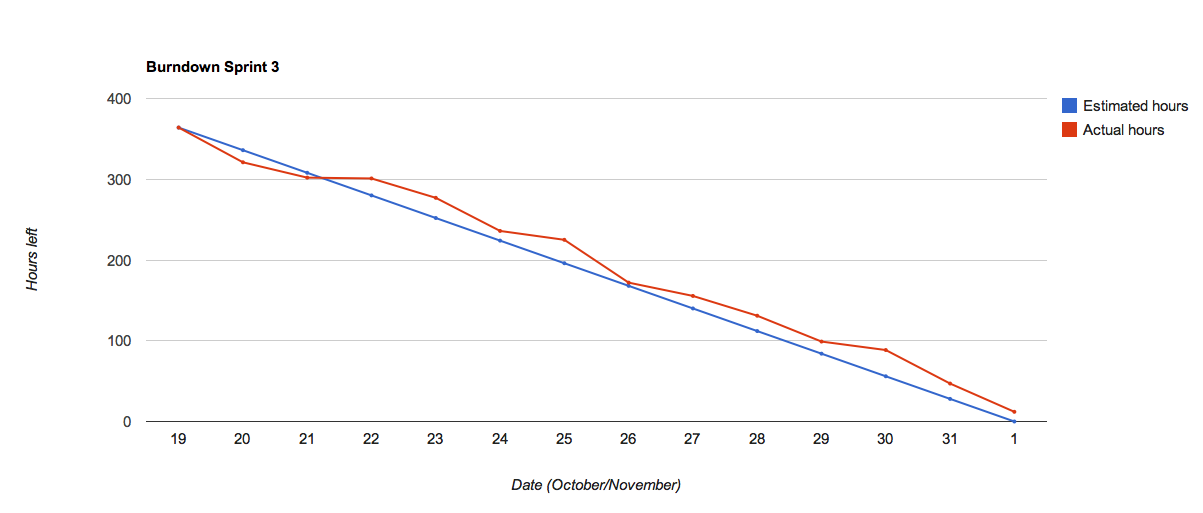
\includegraphics[width=\textwidth]{./sprints/img/burndown_chart_s4}
	\caption{Burndown Chart\label{fig:sp4:burndown}}
\end{figure}

The final testing and patching of the utility had to be done at the customer's site. Two of the team members was assigned to this task. To be allowed to see Thales source code, the team members had to sign a non-disclosure agreement and be under surveillance of the customer. As the customer had a demanding project on their own, they could not spare many hours for the testing.

It took long time to get the security clearance needed, so the testing was blocked until the last week of the sprint. The lack of testing time on the real code, could have ended in a unfinished utility. The lead programmer managed to fix all bugs and make the utility able to parse the source code in the end.

Some of the tasks had to be postponed, until the testing and bug fixing were completed, because of dependencies. 

\subsection{Positive Experiences}
%--------------------------------
\begin{itemize}
	\item We all completed a great amount of work.
	\item Finished all the items in the sprint backlog.
	\item Each team member assigned themselves work items from the backlog, and took responsibility for completing them.
	\item Customer was pleased with our work.
\end{itemize}

\subsection{Negative Experiences}
%--------------------------------
\begin{itemize}
	\item Meetings were ineffective
	\item Stumbled into blocked tasks because of dependencies.
	\item Too few attendants at the stand-up meetings.
\end{itemize}

\subsection{Barriers}
%--------------------

\paragraph{External factors}
The customer asked if we could do a presentation of the utility for the developers at Thales, when it was finished. This would be beneficial for the final presentation and the customer would be pleased, so we accepted. To make the presentation and rehearse for it, two team members had to be excluded from the sprint work for several hours. External factors like this are not always possible to foresee, and it affected the project.

\paragraph{Thales security}
It was necessary to have access to Thales source code for the last test- and bug fixing-phase. As a result of the strict rules at Thales, we had to wait with critical implementation and fixing until the middle of the sprint. We managed to have the utility work on their code in the end.

